\chapter{Homotopy}
To understand an object \(X\) (in our focus, \(X\) denotes topological space), one may try to understand functions
\[
f : A \rightarrow  X, \;\text{ or }\;g : X \rightarrow  B
\]
One special example is to let \(B = \mathbb{R}\). As for two topological spaces, there are many continuous mappings from \(X\) to \(Y\). We will group all these mappings into equivalence classes by checking whether $f$ can be `continuously deformed' to $g$.
\begin{definition} \label{def:homotopy} [Homotopy] A \emph{homotopy} between two continuous maps \(f, g : X \rightarrow  Y\) is a continuous map
\[
H : X \times  \left\lbrack  {0, 1}\right\rbrack   \rightarrow  Y
\]
such that
\[
H\left( {x, 0}\right)  = f\left( x\right), \;H\left( {x, 1}\right)  = g\left( x\right)
\]
If such \(H\) exists, we say \(f\) and \(g\) are homotopic, denoted as 
\[f \simeq  g.\]
\end{definition}
\begin{example} \label{eg:homotopy_convex} Let \(Y \subseteq  {\mathbb{R}}^{2}\) be a convex subset. Consider two continuous maps \(f : X \rightarrow  Y\) and \(g : X \rightarrow  Y\). They are always homotopic since we can define the homotopy
\[
H\left( {x, t}\right)  = {tg}\left( x\right)  + \left( {1 - t}\right) f\left( x\right).
\]
\end{example}

\begin{example} In the picture below, one can take 
\begin{center}
$X = [0,H] \times [0,W]$, $Y = [0,255] \times [0,255] \times [0,255]$ \quad and \quad
$f, g: X \to Y$
\end{center}
$f(h,w) := (r_0,g_0,b_0)$ and $g(h,w) := (r_1,g_1,b_1)$ are the pixels of the leftmost and rightmost picture at coordinate point $(h,w)$ respectively. 

The homotopy $H: X \times [0,1] \to Y$
is a continuous `deformation' of the pixels on the picture. For instance, the pixels of the pictures are continuously deformed by
$$H\left((h,w),0\right) = f(h,w) \ \ \to\ \  H\left((h,w),\frac{1}{3}\right)\ \ \to\ \  H\left((h,w),\frac{2}{3}\right) \ \ \to\ \ H\left((h,w),1\right) = g(h,w).$$
\begin{center}
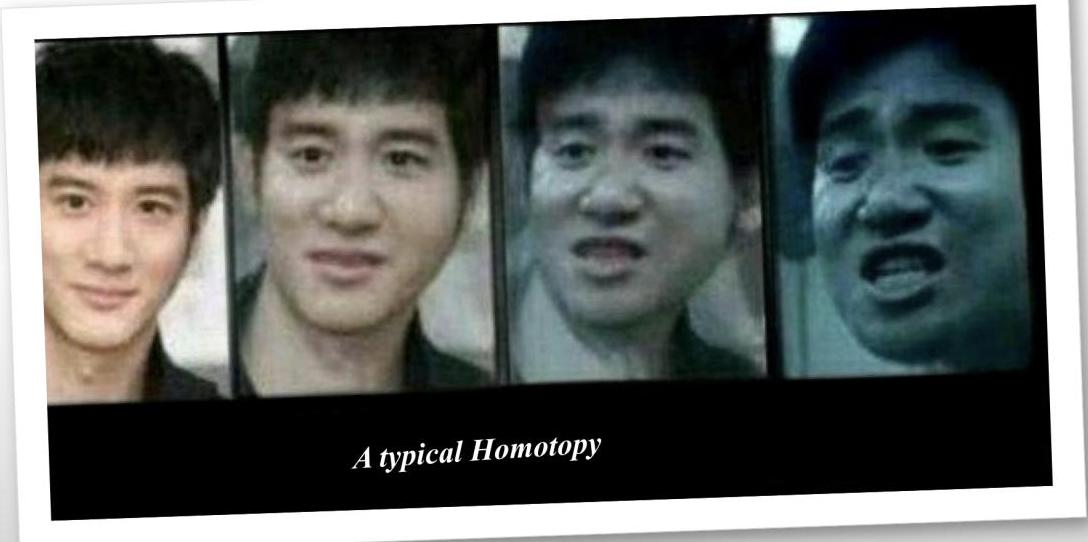
\includegraphics[width=0.8\textwidth]{images/Ch5_Cheung.jpg}
\end{center}
\end{example}

\begin{proposition} Homotopy is an equivalence relation.
\end{proposition}

\begin{proof} 1. Let \(f : X \rightarrow  Y\) be any continuous map. Then \(f \simeq  f\) : we can define a homotopy \(H\left( {x, t}\right)  = f\left( x\right), \forall 0 \leq  t \leq  1\).

2. Suppose \(f \simeq  g\), i.e., \(H\) is a homotopy between \(f\) and \(g\), then \(g \simeq  f\) : Define the mapping \({H}^{\prime }\left( {x, t}\right)  = H\left( {x, 1 - t}\right)\), then
\[
{H}^{\prime }\left( {x, 0}\right)  = g\left( x\right), \;{H}^{\prime }\left( {x, 1}\right)  = f\left( x\right)
\]

3. Let \(f, g, h : X \rightarrow  Y\) be three continuous maps. If \(f\) and \(g\) are homotopic and \(g\) and \(h\) are homotopic, then \(f\) and \(h\) are homotopic: Let \(H : X \times  \left\lbrack  {0, 1}\right\rbrack   \rightarrow  Y\) be a continuous map such that
\[
H\left( {x, 0}\right)  = f\left( x\right), H\left( {x, 1}\right)  = g\left( x\right) ;
\]
\(K : X \times  \left\lbrack  {0, 1}\right\rbrack   \rightarrow  Y\) be a continuous map such that
\[
K\left( {x, 0}\right)  = g\left( x\right), K\left( {x, 1}\right)  = h\left( x\right).
\]
Define a function \(J : X \times  \left\lbrack  {0, 1}\right\rbrack   \rightarrow  Y\) by
\[
J\left( {x, t}\right)  = \left\{  \begin{matrix} H\left( {x, {2t}}\right), & 0 \leq  t \leq  1/2 \\  K\left( {x, {2t} - 1}\right), & 1/2 \leq  t \leq  1 \end{matrix}\right.
\]
Then \(J\) is continuous, since for all closed \(V \subseteq  Y\), 
\[
{J}^{-1}\left( V\right)  = \left( {{J}^{-1}\left( V\right)  \cap  \left( {X \times  \left\lbrack  {0, 1/2}\right\rbrack  }\right) }\right)  \cup  \left( {{J}^{-1}\left( V\right)  \cap  \left( {X \times  \left\lbrack  {1/2, 1}\right\rbrack  }\right) }\right)  = {H}^{-1}\left( V\right)  \cup  {K}^{-1}\left( V\right), 
\]
and the closedness of \({H}^{-1}\left( V\right)\) and \({K}^{-1}\left( V\right)\) implies the closedness of \({J}^{-1}\left( V\right)\).

Moreover, \(J\) has the property that \(J\left( {x, 0}\right)  = H\left( {x, 0}\right)  = f\left( x\right)\), while \(J\left( {x, 1}\right)  =\)  \(K\left( {x, 1}\right)  = h\left( x\right)\).
\end{proof}


Back to \autoref{eg:homotopy_convex}: If \(Y \subseteq  {\mathbb{R}}^{n}\) is convex, then the set of continuous functions \(f : X \rightarrow  Y\) form a single equivalence class. In other words, all such maps are homotopic to each other.

\begin{proposition} \label{prop:comp_homotopy} Consider four continuous mappings
\[
W\overset{f}{ \rightarrow  }X, \;X\overset{g}{ \rightarrow  }Y, \;X\overset{h}{ \rightarrow  }Y, \;Y\overset{k}{ \rightarrow  }Z.
\]
If \(g \simeq  h\), then
\[
g \circ  f \simeq  h \circ  f, \;k \circ  g \simeq  k \circ  h
\]
\end{proposition}
\begin{proof} Suppose there exists the homotopy \(H : g \simeq  h\), then \(k \circ  H : X \times  I \rightarrow  Z\) gives the homotopy between \(k \circ  g\) and \(k \circ  h\).

Similarly, \(H \circ  \left( {f \times  {\operatorname{id}}_{I}}\right)  : W \times  I \rightarrow  Y\) gives the homotopy \(g \circ  f \simeq  h \circ  f\).
\end{proof}

\begin{definition} \label{def:homotopy_equivalence} [Homotopy Equivalence] Two topological spaces \(X\) and \(Y\) are homotopy equivalent if there are continuous maps \(f : X \rightarrow  Y\), and \(g : Y \rightarrow  X\) such that
\begin{align*}
g \circ  f &\simeq  {\operatorname{id}}_{X \rightarrow  X}
\\
f \circ  g &\simeq  {\operatorname{id}}_{Y \rightarrow  Y}, 
\end{align*}
which is denoted as \(X \simeq  Y\). 
\end{definition}

\begin{proposition}
Let $X$ and $Y$ be topological spaces.
\begin{enumerate}
    \item If \(X \cong  Y\) are homeomorphic, then they are homotopic equivalent.
    \item The homotopy equivalence \(X \simeq  Y\) gives a bijection between \(\{ \phi  :\) continuous \(W \rightarrow\)  \(X\} / \sim\) and \(\{ \phi\) : continuous \(W \rightarrow  Y\} / \sim\), for any given topological space \(W\).
    \item The homotopy equivalence \(X \simeq  Y\) forms an equivalence relation between topological spaces.
\end{enumerate}
\end{proposition}

\begin{proof} Since \(X \simeq  Y\), we can find \(f : X \rightarrow  Y\) and \(g : Y \rightarrow  X\) such that \(f \circ  g \simeq\)  \({\mathrm{{id}}}_{Y}\) and \(g \circ  f \simeq  {\mathrm{{id}}}_{X}\). We construct a mapping
\[\alpha  : \;\{ \phi  : W \rightarrow  X\ | \ \phi \text{ continuous}\} / \sim \ \longrightarrow  \{ \phi  : W \rightarrow  Y\ | \ \phi \text{ continuous}\} / \sim\]
by \(\left\lbrack  \phi \right\rbrack   \mapsto  \left\lbrack  {f \circ  \phi }\right\rbrack\). Then one can check \(\alpha\) is well-defined, since \({\phi }_{1} \sim  {\phi }_{2}\) implies \(f \circ  {\phi }_{1} \sim  f \circ  {\phi }_{2}\).

Also, we can construct a mapping
\[\beta  : \;\{ \phi  :W \rightarrow  Y\ | \ \phi \text{ continuous}\} / \sim \  \longrightarrow  \{ \phi  :W \rightarrow  X\ | \ \phi \text{ continuous}\} / \sim\]
by \(\left\lbrack  \psi \right\rbrack   \mapsto  \left\lbrack  {g \circ  \phi }\right\rbrack\). Similarly, \(\beta\) is well-defined.

Now one can check that \(\alpha  \circ  \beta  = \mathrm{{id}}\) and \(\beta  \circ  \alpha  = \mathrm{{id}}\). For example, 
\[
\alpha  \circ  \beta \left\lbrack  \psi \right\rbrack   = \left\lbrack  {f \circ  g \circ  \psi }\right\rbrack   = \left\lbrack  \psi \right\rbrack , 
\]
where the last equality is due to the fact that \(f \circ  g \simeq  {\operatorname{id}}_{Y}\).

3. is left as an exercise.
\end{proof}

Compared with homeomorphism, some properties are lost when we consider homotopy equivalence.
\begin{definition} \label{def:contractible} [Contractible] The topological space \(X\) is \emph{contractible} if it is homotopy equivalent to any point \(\{ \mathbf{c}\}\).

In other words, there exists continuous mappings \(f, g\) such that
\[
\{ \mathbf{c}\} \overset{f}{ \rightarrow  }X\overset{g}{ \rightarrow  }\{ \mathbf{c}\}, g \circ  f \simeq  {\operatorname{id}}_{\{ \mathbf{c}\} }
\]
\[
X\overset{g}{ \rightarrow  }\{ \mathbf{c}\} \overset{f}{ \rightarrow  }X, f \circ  g \simeq  {\operatorname{id}}_{X}
\]
\end{definition}

Note that \(g \circ  f \simeq  {\operatorname{id}}_{\{ c\} }\) follows naturally; and since \(X \cong  X\), we can find \(f, g\) such that \(f \circ  g = {c}_{y}\) for some \(y \in  X\), where \({c}_{y} : X \rightarrow  X\) is a constant function \({c}_{y}\left( x\right)  = y, \forall x \in  X\). Therefore, to check \(X\) is contractible, it suffices to check \({c}_{y} \simeq  {\operatorname{id}}_{X}, \forall y \in  X\) Therefore, \(X\) is contractible if its identity map \({\operatorname{id}}_{X}\) is homotopic to any constant map \({c}_{y}, \forall y \in  X\).

\begin{proposition} The definition for $X$ being contractible can be simplified further:

1. \(X\) is contractible if it is homotopy equivalent to some point \(\{ c\}\)

2. \(X\) is contractible if the identity map \({\operatorname{id}}_{X}\) is homotopic to some constant map
\[
{c}_{y}\left( x\right)  = y.
\]
\end{proposition}

\begin{proof} The only thing is to show that \({c}_{y} \simeq  {c}_{{y}^{\prime }}, \forall y, {y}^{\prime } \in  X\). By homework 3, \(X\) is path-connected, and therefore there exists continuous \(p\left( t\right)\) such that
\[
p\left( 0\right)  = y, \;p\left( 1\right)  = {y}^{\prime }
\]
Therefore, we construct the homotopy between \({c}_{y}\) and \({c}_{{y}^{\prime }}\) as follows:
\[
H\left( {x, t}\right)  = p\left( t\right).
\]
\end{proof}

\begin{example} \(X = {\mathbb{R}}^{2}\) is contractible:
It suffices to show that the mapping \(f\left( \mathbf{x}\right)  = \mathbf{x}, \forall \mathbf{x} \in  {\mathbb{R}}^{2}\) is homotopic to the constant function \(g\left( x\right)  = \left( {0, 0}\right), \forall x \in  {\mathbb{R}}^{2}\), i.e., \(g = {c}_{\left( 0, 0\right) }\).

Consider the continuous mapping \(H\left( {\mathbf{x}, t}\right)  = {tf}\left( \mathbf{x}\right)\), with
\[
H\left( {\mathbf{x}, 0}\right)  = {c}_{\left( 0, 0\right) }, \;H\left( {\mathbf{x}, 1}\right)  = {\operatorname{id}}_{X}
\]
Therefore, \({c}_{\left( 0, 0\right) } \simeq  {\mathrm{{id}}}_{X}\). Since \({c}_{\left( 0, 0\right) } \simeq  {c}_{\mathbf{y}}, \forall \mathbf{y} \in  {\mathbb{R}}^{2}\), we imply \({c}_{\mathbf{y}} \simeq  {\mathrm{{id}}}_{X}\) for any \(\mathbf{y} \in  {\mathbb{R}}^{2}\). Therefore, \(X\) is contractible. More generally, any convex \(X \subseteq  {\mathbb{R}}^{n}\) is contractible.
\end{example}

\begin{remark}
\({S}^{1}\) is not contractible, and we will see later. In particular, we are not able to construct the continuous mapping
\[
H : {S}^{1} \times  \left\lbrack  {0, 1}\right\rbrack   \rightarrow  {S}^{1}
\]
such that
\[
H\left( {{e}^{2\pi ix}, 0}\right)  = {e}^{2\pi ix}, \;H\left( {{e}^{2\pi ix}, 1}\right)  = {e}^{{2\pi i}\left( 0\right) } = 1
\]
One may ask - how about the mapping \(H\left( {{e}^{2\pi ix}, t}\right)  = {e}^{2\pi ixt}\)? Unfortunately, it is not well-defined, since
\[
H\left( {{e}^{{2\pi i}\left( 1\right) }, t}\right)  = {e}^{2\pi it} = H\left( {{e}^{{2\pi i}\left( 0\right) }, t}\right)  = 1
\]
and the equality is not true for \(t \neq  0, 1\).
\end{remark}

\begin{definition} \label{def:homotopy_retract} [Homotopy Retract] Let \(A \subseteq  X\) and \(i : A \hookrightarrow  X\) be an inclusion. We say \(A\) is a \emph{homotopy retract} of \(X\) if there exists continuous mapping \(r : X \rightarrow  A\) such that
\[
r \circ  i : A \hookrightarrow  X\overset{r}{ \rightarrow  }A = {\operatorname{id}}_{A}
\]
\[
i \circ  r : X\overset{r}{ \rightarrow  }A \hookrightarrow  X \simeq  {\operatorname{id}}_{X}
\]
In particular, \(A \simeq  X\).
\end{definition}
\begin{example} The $1$-sphere \({S}^{1}\) is a homotopy retract of Mobius band \(M\). More explicitly, 
let \(M = {\left\lbrack  0, 1\right\rbrack  }^{2}/ \sim\) and \({S}^{1} = \left\lbrack  {0, 1}\right\rbrack  / \sim\) by the appropriate equivalence relations. Then the inclusion \(i\) and the retraction \(r\) are given by:
\[i(\left\lbrack  x\right\rbrack)  :=  \left\lbrack  \left( {x, \frac{1}{2}}\right) \right\rbrack
\]
\[r\left\lbrack  \left( {x, y}\right) \right\rbrack  :=  \left\lbrack  x\right\rbrack
\]
As a result, 
\[
r \circ  i = {\operatorname{id}}_{{S}^{1}}, \;i \circ  r\left( \left\lbrack  \left( {x, y}\right) \right\rbrack  \right)  = \left\lbrack  \left( {x, 1/2}\right) \right\rbrack
\]
It suffices to show \(i \circ  r \simeq  {\mathrm{{id}}}_{M}\), where \({\mathrm{{id}}}_{M}\left( \left\lbrack  \left( {x, y}\right) \right\rbrack  \right)  = \left\lbrack  \left( {x, y}\right) \right\rbrack\).
To do so, construct the continuous mapping \(H : M \times  I \rightarrow  M\) with
\[
H\left( {\left\lbrack  \left( {x, y}\right) \right\rbrack , t}\right)  \mathrel{\text{ := }} \left\lbrack  \left( {x, \left( {1 - t}\right) y + t/2}\right) \right\rbrack
\]
To show the well-definedness of \(H\), we need to check
\[
H\left( {\left\lbrack  \left( {0, y}\right) \right\rbrack , t}\right)  = H\left( {\left\lbrack  \left( {1, 1 - y}\right) \right\rbrack , t}\right), \;\forall y \in  \left\lbrack  {0, 1}\right\rbrack
\]
It’s clear that \(H\) gives a homotopy between \(i \circ  r\) and \({\mathrm{{id}}}_{M}\), i.e., \(i \circ  r \simeq  {\mathrm{{id}}}_{M}\)
\end{example}

\begin{example} The \(n - 1\) -sphere \({S}^{n - 1}\) is a homotopy retract of \({\mathbb{R}}^{n} \smallsetminus  \{ \mathbf{0}\}\): Consider the usual inclusion \(i : {S}^{n - 1} \rightarrow  {\mathbb{R}}^{n} \smallsetminus  \{ 0\}\) and
\[
r : \;{\mathbb{R}}^{n} \smallsetminus  \{ 0\}  \rightarrow  {\mathbb{S}}^{n - 1}
\]
with $r(x) = \frac{x}{\parallel x\parallel }$. Therefore, \(r \circ  i = {\operatorname{id}}_{{S}^{n - 1}}\) and \(i \circ  r\left( x\right)  = \frac{x}{\parallel x\parallel }\).

It suffices to show that \(i \circ  r \simeq  {\operatorname{id}}_{{\mathbb{R}}^{n}\smallsetminus \{ 0\} }\). To see so, consider the homotopy 
\[H\left( {x, t}\right)  = {tx} + (1 -t)\mathbf{x}/\parallel \mathbf{x}\parallel.\] 
Then $H$ is well-defined, since \(H\left( {x, t}\right)  \in  {\mathbb{R}}^{n} \smallsetminus  \{ \mathbf{0}\}\) for all \(\mathbf{x} \in  {\mathbb{R}}^{n} \smallsetminus  \{ \mathbf{0}\}\) and \(t \in  \left\lbrack  {0, 1}\right\rbrack\).

Note that 
\[
H\left( {\mathbf{x}, 0}\right)  = i \circ  r\left( \mathbf{x}\right), \;H\left( {\mathbf{x}, 1}\right)  = \mathbf{x} = \operatorname{id}\left( \mathbf{x}\right)
\]
so the result follows.
\end{example}

\begin{definition} \label{def:relative_homotopy} [Homotopic Relative] Let \(A \subseteq  X\) be topological spaces. We say \(f, g : X \rightarrow  Y\) are homotopic relative to \(A\) if there exists \(H : X \times  I \rightarrow  Y\) such that
\[
\left\{  {\begin{array}{l} H\left( {x, 0}\right)  = f\left( x\right) \\  H\left( {x, 1}\right)  = g\left( x\right)  \end{array}\;\text{ and }H\left( {a, t}\right)  = f\left( a\right)  = g\left( a\right), \forall a \in  A}\right.
\]
\end{definition}

\section{Simplicial Approximation Theorem}
In this section, we wish to understand homotopy between simplicial complexes \(f, g : \left| K\right|  \rightarrow  \left| L\right|\)

\begin{definition} [Simplicial Map] A simplicial map between \({K}_{1} = \left( {{V}_{1}, {\sum }_{1}}\right)\) and \({K}_{2} =\)  \(\left( {{V}_{2}, {\sum }_{2}}\right)\) is a mapping \(f : {K}_{1} \rightarrow  {K}_{2}\) such that

1. It maps vertices to vertices

2. It maps simplicies to simplicies, i.e., 
\[
f\left( {\sigma }_{1}\right)  \in  {\sum }_{2}, \forall {\sigma }_{1} \in  {\sum }_{1}, 
\]
\end{definition}

\begin{example} Consider the simplicial complexes defined as follows:
\begin{center}
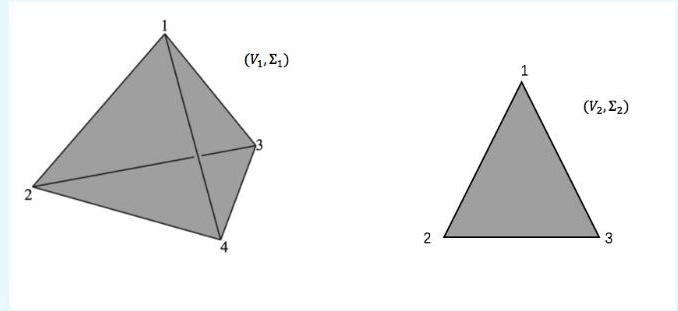
\includegraphics[width=0.5\textwidth]{images/Ch5_simplex_map.jpg}
\end{center}
In particular, \(\{ 1, 2, 3, 4\}  \notin  {\sum }_{1}\) and \(\{ 1, 2, 3\}  \in  {\sum }_{2}\). Then we can define the simplicial map as:
\[
f\left( 1\right)  = 1, \;f\left( 2\right)  = 2, \;f\left( 3\right)  = 3, \;f\left( 4\right)  = 3
\]
In particular, \(f\left( {\{ 1, 2, 4\} }\right)  = \{ 1, 2, 3\}  \in  {\sum }_{2}\).
\end{example}

Now we want to define the simplicial map between the topological realizations. There are several observations:
\begin{enumerate}
\item We have seen that each \(\left| K\right|  \subseteq  {\mathbb{R}}^{m}\) for some \(m\). In particular, \(m = \# V - 1\).

\item Each point \(x \in  \left| K\right|\) lies uniquely on an inside of some \({\Delta }_{\sigma }\), , where \(\sigma  \in  \sum\).

\item Suppose that the vertices of \({K}_{1}\) are \({V}_{1} = \left\{  {{u}_{1}, \ldots, {u}_{n}}\right\}   \subseteq  {\mathbb{R}}^{m}\). Then every \(\mathbf{x} \in  {K}_{1}\) can be uniquely written as
\[
\mathbf{x} = \mathop{\sum }\limits_{{i = 1}}^{k}{\alpha }_{i}{U}_{{\sigma }_{i}}
\]
with \({\alpha }_{i} > 0, \sum {\alpha }_{i} = 1\) and \(\sigma  = \left\{  {{U}_{{\sigma }_{1}}, \ldots, {U}_{{\sigma }_{k}}}\right\}\) is the unique simplex where \(x \in\) inside \(\left( {\Delta }_{\sigma }\right)\).
\begin{center}
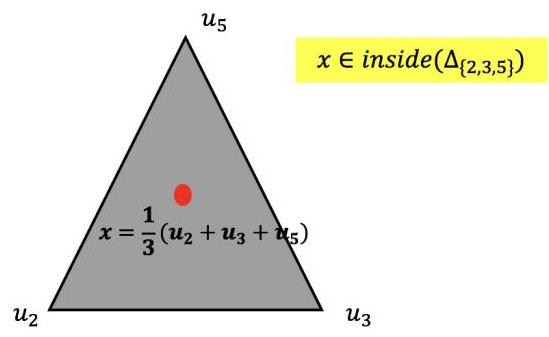
\includegraphics[width=0.4\textwidth]{images/Ch5_inside_coords.jpg}
\end{center}
\item Our simplicial map \(f\) maps \({V}_{1}\) to \({V}_{2} = \left\{  {{w}_{1}, \ldots, {w}_{p}}\right\}   \subseteq  {\mathbb{R}}^{m}\), so for each \(i\), we have \(f\left( {\mathbf{u}}_{i}\right)  = {\mathbf{w}}_{j}\) for some \(j \in  \{ 1, \ldots, p\}.\)
\end{enumerate}

\begin{definition} [Mapping induced from Simplicial Mapping] The simplicial map \(f : {K}_{1} \rightarrow\)  \({K}_{2}\) induces a mapping \(\left| f\right|  : \left| {K}_{1}\right|  \rightarrow  \left| {K}_{2}\right|\) between the topological realizations such that

\begin{enumerate}
    \item It maps vertexes to vertexes, i.e., \(\left| f\right| \left( {v}_{1}\right)  = f\left( {v}_{1}\right), \forall {v}_{1} \in  V\left( {K}_{1}\right)\).

\item it is affine, i.e., 
\[
\left| f\right| \left( {\mathop{\sum }\limits_{{i = 1}}^{k}{\alpha }_{i}{v}_{i}}\right)  = \mathop{\sum }\limits_{{i = 1}}^{k}{\alpha }_{i}\left| f\right| \left( {v}_{i}\right)
\]
\end{enumerate}
(note that \(\left| f\right|  : \left| {K}_{1}\right|  \rightarrow  \left| {K}_{2}\right|\) is continuous).
\end{definition}

Here is our more refined goal: Suppose we are given a continuous map \(\left| g\right|  : \left| K\right|  \rightarrow  \left| L\right|\), we want to approximate \(\left| g\right|\) by \(\left| f\right|\), where \(f : K \rightarrow  L\) is a simplicial map. It is obvious that \(f\) is an easier object to study compared with \(\left| g\right|\).

However, we cannot achieve this goal unless we subdivide \(K\) into smaller pieces:

\begin{definition} [Subdivision] Let \(K\) be a simplicial complex. A simplicial complex \({K}^{\prime }\) is called a \emph{subdivision} of \(K\) if

\begin{enumerate}
    \item Each simplex of \({K}^{\prime }\) is contained in a simplex of \(K\)

\item Each simplex of \(K\) equals the union of finitely many simplices of \({K}^{\prime }\)
\end{enumerate} 
As a result, we can form an homeomorphism \(h : \left| {K}^{\prime }\right|  \rightarrow  \left| K\right|\) such that for each \({\sigma }^{\prime } \in  {\sum }_{{K}^{\prime }}\), there exists \(\sigma  \in  {\sum }_{K}\) satisfying
\[
f\left( {\Delta }_{{\sigma }^{\prime }}\right)  \in  {\Delta }_{\sigma }
\]
\end{definition}

\begin{example} Consider the map \(\left| g\right|  : \left| K\right|  \rightarrow  \left| L\right|\) given in the figure below:
\begin{center}
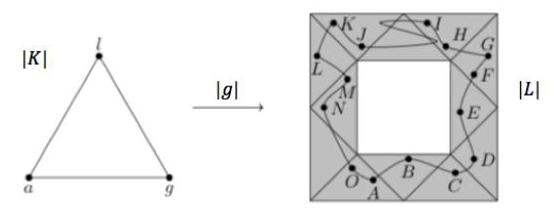
\includegraphics[width=0.6\textwidth]{images/Ch5_no_simplicial_map.jpg}
\end{center}
where \(\left| g\right| \left( a\right) = A\), \(\left| g\right| \left( g\right) = G\) and \(\left| g\right| \left( l\right) = L\). It is clear that we cannot find a 
simplicial map $\gamma: K \to L$ such that $|\gamma| = |g|$, since (for instance) the $1$-simplex $\Delta_{\{a,l\}}$ of $K$ does not lie in a single simplex $\Delta_{\sigma}$ of $L$. 

To remedy this, we subdivide \(K\) into smaller pieces as follows:
\begin{center}
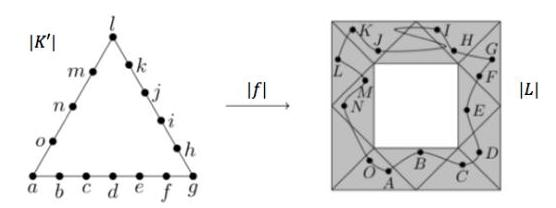
\includegraphics[width=0.6\textwidth]{images/Ch5_subdivide_map.jpg}
\end{center}
In this case, it is clear that 
one can define a simplicial map $f:K' \to L$ such that
\(\left| f\right|  : \left| {K}^{\prime }\right|  \rightarrow  \left| L\right|\) is our original map on the topological spaces.
\end{example}

\begin{example} [Barycentric Subdivision] One typical subdivision is the \emph{barycentric subdivision}. Namely, for each simplicial complex $K$, we add extra vertices, which corresponds to the barycenters of the topological realization of $K$. One example of such subdivision is given below:
\begin{center}
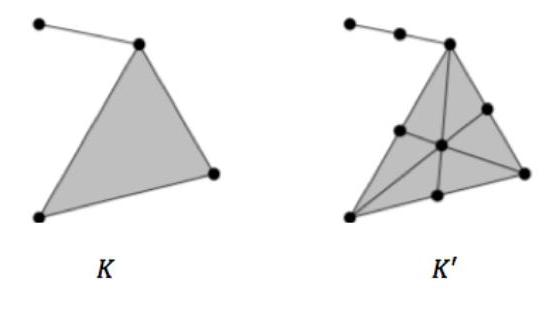
\includegraphics[width=0.5\textwidth]{images/Ch5_barycentric.jpg}
\end{center}
\end{example}

\begin{remark} Suppose we have a metric on \(\left| K\right|\). By subdivision, we can consider \(\left| {K}^{\prime }\right|\) such that for any \({\sigma }^{\prime } \in  {\sum }_{{K}^{\prime }}\), any two points in \({\Delta }_{{\sigma }^{\prime }}\) has a smaller distance.
\end{remark}

The following result gives a criterion for the existence of a simplicial approximation for a mapping between topological realizations. For this we recall the notion of star at a vertex \(v\) of $K$:
\[
\operatorname{star}\left( v\right)  = \mathop{\bigcup }\limits_{{v \in  \sigma }}{\sigma }^{ \circ  }.
\]

\begin{proposition} \label{prop:simplicial_approx} Let \(f : \left| K\right|  \rightarrow  \left| L\right|\) be a continuous mapping. Suppose that for each \(v \in  {V}_{K}\), there exists \(g\left( v\right)  \in  {V}_{L}\) such that
\[
f\left( {{\operatorname{st}}_{K}\left( v\right) }\right)  \subseteq  {\operatorname{st}}_{L}\left( {g\left( v\right) }\right)
\]
then the mapping \(g : {V}_{K} \rightarrow  {V}_{K}\) gives \(\left| g\right|  \simeq  f\). In such a case, \(g\) is called a {\bf simplicial approximation} to \(f\).
\end{proposition}

\begin{example} 
Let $K$ is as given below:
\begin{center}
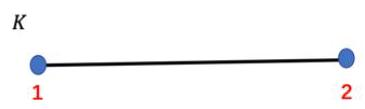
\includegraphics[width=0.3\textwidth]{images/Ch5_line_K.jpg}
\end{center}
If the map $f:|K| \to |L|$ is given by:
\begin{center}
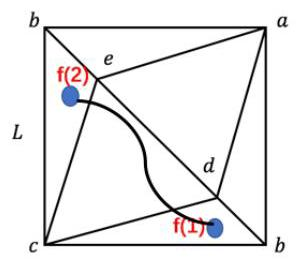
\includegraphics[width=0.4\textwidth]{images/Ch5_no_simp_K.jpg}
\end{center}
\hspace*{3em} 
The hypothesis of \autoref{prop:simplicial_approx} is not satisfied, so we cannot apply this proposition to construct a simplicial map $g: K \to L$ such that $|g| \simeq f$ (and indeed there is no such $g$).

However, if we subdivide $K$ into smaller parts (5 in the picture below): 
\begin{center}
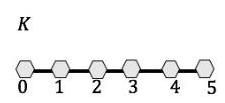
\includegraphics[width=0.4\textwidth]{images/Ch5_5_segments.jpg}
\end{center}
and $f:|K| \to |L|$ is given by:
\begin{center}
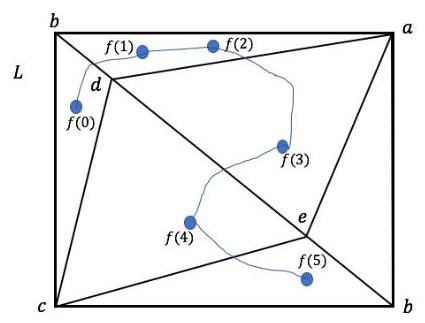
\includegraphics[width=0.4\textwidth]{images/Ch5_example_simplicial_approx.jpg}
\end{center}
then \autoref{prop:simplicial_approx} is satisfied. In such a case, 
we can take a simplicial approximation \(g\) by
\[
g\left( 0\right)  = b, g\left( 1\right)  = g\left( 2\right)  = d, g\left( 3\right)  = e, g\left( 4\right)  = c, g\left( 5\right)  = b.
\]
\end{example}

\begin{proof} We first show a statement: Suppose that \(\sigma  = \left\{  {{v}_{0}, \ldots, {v}_{n}}\right\}   \in  \sum \left( K\right)\), and \(x \in\) inside \(\left( \sigma \right)  \subseteq  \left| K\right|\). If \(f\left( x\right)  \in  \left| L\right|\) lies in the inside of the (unique) simplex \(\tau  \in  {\sum }_{L}\), (i.e., \(f\left( x\right)\) can uniquely be expressed as \(\mathop{\sum }\limits_{{{u}_{i} \in  \tau }}{\beta }_{i}{u}_{i}\), such that \({\beta }_{i} > 0, \forall i\) and \(\left. {\mathop{\sum }\limits_{i}{\beta }_{i} = 1}\right)\) then \(g\left( {v}_{0}\right), \ldots, g\left( {v}_{n}\right)\) are vertices of \(\tau\).

By definition of inside \(\left( \sigma \right), x = \mathop{\sum }\limits_{{i = 0}}^{n}{\alpha }_{i}{v}_{i}\) with \({\alpha }_{i} > 0\) and \(\mathop{\sum }\limits_{{i = 1}}^{n}{\alpha }_{i} = 1\). Therefore, \(x \in  {\operatorname{st}}_{K}\left( {v}_{i}\right)\) for \(i = 1, \ldots, n\), where

\[
{\operatorname{st}}_{K}\left( {v}_{i}\right)  \mathrel{\text{ := }} \left\{  {a{v}_{i} + \mathop{\sum }\limits_{{j = 1}}^{m}{b}_{j}{w}_{j} \mid  a > 0, {b}_{j} > 0, a + \mathop{\sum }\limits_{{j = 1}}^{m}{b}_{j} = 1, \left\{  {{v}_{i}, {w}_{1}, \ldots, {w}_{m}}\right\}   \in  {\sum }_{K}}\right\} .
\]

Therefore, \(f\left( x\right)  \in  \operatorname{int}\left( {{\operatorname{st}}_{K}\left( {v}_{i}\right) }\right)  \subseteq  {\operatorname{st}}_{L}\left( {g\left( {v}_{i}\right) }\right)\), which follows that

\[
f\left( x\right)  = {ag}\left( {v}_{i}\right)  + \mathop{\sum }\limits_{{j = 1}}^{m}{b}_{j}{u}_{j}, \text{ where }a > 0, {b}_{j} > 0, a + \mathop{\sum }\limits_{{j = 1}}^{m}{b}_{j} = 1, \left\{  {g\left( {v}_{i}\right), {u}_{1}, \ldots, {u}_{m}}\right\}   \in  {\sum }_{L}
\]

Comparing the above formula with our hypothesis on \(f\left( x\right), g\left( {v}_{i}\right)\) is a vertex of the simplex \(\tau, i = 1, \ldots, n\). Moreover, \(\left\{  {g\left( {v}_{0}\right), \ldots, g\left( {v}_{n}\right) }\right\}\) is a subset of \(\tau\), which is a face of \(\tau\), and therefore \(\left\{  {g\left( {v}_{0}\right), \ldots, g\left( {v}_{n}\right) }\right\}   \in  {\sum }_{L}\).

\begin{itemize}
\item Therefore, the mapping \(g : K \rightarrow  L\) maps simplicies to simplicies, which is a simplicial mapping. We can construct a homotopy between \(f\) and \(\left| g\right|\) as follows: Consider any \(x \in  \left| K\right|\), and let \(\tau  \in  {\sum }_{L}\) be such that \(f\left( x\right)  \in  \operatorname{inside}\left( \tau \right)\). We write \(x = \mathop{\sum }\limits_{{i = 0}}^{n}{\lambda }_{i}{v}_{i}\) for some \(\left\{  {{v}_{0}, \ldots, {v}_{n}}\right\}   \in  {\sum }_{K}\) and \({\lambda }_{i} > 0, \mathop{\sum }\limits_{{i = 1}}^{n}{\lambda }_{i} = 1\). Applying our claim, 
\end{itemize}

\[
\left| g\right| \left( x\right)  = \mathop{\sum }\limits_{{i = 0}}^{n}{\lambda }_{i}g\left( {v}_{i}\right), 
\]

where \(g\left( {v}_{0}\right), \ldots, g\left( {v}_{n}\right)\) are all vertices of \(\tau\).

We can directly construct a homotopy between \(f\) and \(\left| g\right|\). Before that, we need some reformulations. Since \(f\left( x\right)  \in  \operatorname{inside}\left( \tau \right)\), we let \(f\left( x\right)  = \mathop{\sum }\limits_{{i = 0}}^{m}{\mu }_{i}{\tau }_{i}\). Since \(\left| g\right| \left( x\right)  =\)  \(\mathop{\sum }\limits_{{i = 0}}^{n}{\lambda }_{i}g\left( {v}_{i}\right)  \in  \operatorname{inside}\left( \tau \right)\), we rewrite \(\left| g\right| \left( x\right)  = \mathop{\sum }\limits_{{i = 0}}^{m}{\lambda }_{i}^{\prime }{\tau }_{i}\). (by adding some \({\lambda }_{i}^{\prime } \mathrel{\text{ := }} 0\) if necessary) We define the map

\[
H : \;\left| K\right|  \times  I \rightarrow  \left| L\right|
\]

\[
\text{ with }\left( {x, t}\right)  \mapsto  \mathop{\sum }\limits_{{i = 0}}^{m}t{\lambda }_{i}^{\prime } + \left( {1 - t}\right) {\mu }_{i}
\]

which follows that \(f \simeq  \left| g\right|\).
\end{proof}

\begin{theorem} \label{thm:simplicial_approx}[Simplicial Approximation Theorem] Let \(K, L\) be simplicial complexes with \({V}_{K}\) finite, and \(f : \left| K\right|  \rightarrow  \left| L\right|\) be continuous. Then there exists a subdivision \(\left| {K}^{\prime }\right|\) of \(\left| K\right|\) together with a simplicial map \(g\) such that \(\left| g\right|  \simeq  f\).

Here the way for constructing subdivision \(\left| {K}^{\prime }\right|\) is as follows. There exists a constant \(\delta  > 0\). As long as the coarseness of \({K}^{\prime }\) is less than \(\delta\), our constructed subdivision satisfies the condition.
\end{theorem}


Proof. The sets \(\left\{  {{\operatorname{st}}_{L}\left( w\right)  \mid  w \in  V\left( L\right) }\right\}\) forms an open cover of \(\left| L\right|\), which implies \(\left\{  {{f}^{-1}\left( {{\operatorname{st}}_{L}\left( w\right) }\right) }\right\}\) forms an open cover of \(\left| K\right|\). By compactness, there exists a finite subcover of \(\left| K\right|\), denoted as

\[
\left| K\right|  \subseteq  \mathop{\bigcup }\limits_{{i = 1}}^{n}{f}^{-1}\left( {{\operatorname{st}}_{L}\left( {w}_{i}\right) }\right)
\]

There exists a small number \(\delta  > 0\) such that for any \(x, y \in  \left| K\right|\) with \(d\left( {x, y}\right)  < \delta\), \(x, y \in  {f}^{-1}\left( {{\operatorname{st}}_{L}\left( {w}_{i}\right) }\right)\) for some \(i\). Then we construct a simplicial subdivision \(\left| {K}^{\prime }\right|\) of \(\left| K\right|\) with coarseness less than \(\delta\), i.e., \(\forall x, y \in  {\operatorname{st}}_{{K}^{\prime }}\left( v\right), d\left( {x, y}\right)  < \delta\).

Therefore, \({\operatorname{st}}_{{K}^{\prime }}\left( v\right)  \subseteq  {f}^{-1}\left( {{\operatorname{st}}_{L}\left( {w}_{i}\right) }\right)\) for any \(v \in  V\left( K\right)\) and some \({w}_{i} \in  V\left( L\right)\), i.e., \(f\left( {{\operatorname{st}}_{{K}^{\prime }}\left( v\right) }\right)  \subseteq\)  \({\operatorname{st}}_{L}\left( {w}_{i}\right)\).